\section{Arquitectura funcional}

\subsection{consideraciones para generar la arquitectura funcional}
\begin{enumerate}
    \item Las funciones deben ser claras.
    \item Entender la conexión y comunicación entre funciones. 
\end{enumerate}

\subsection{Esta compuesta por los siguientes tres modelos}
\begin{enumerate}
    \item Jerarquía de funciones (FBS: Function, Behaviour, Structure)
    \item Relación entre funciones (IDEF-0: Integration Definition for Function Modeling)
    \item Comportamiento ente funciones (EFFBD: Enhanced Function Flow Block Diagram)
\end{enumerate}

Considerando los atributos de sistemas mecatrónicos, y las funciones generales del sistema propuesto. Las funciones genéricas del sistema mecatrónico son:
\begin{itemize}
    \item F10: Medición de parámetros del sistema y entorno.
    \item F20: Detección de errores del sistema.
    \item F30: Interacción con el usuario.
    \item F40: Administración de decisiones, proceso de aprendizaje, manejo del conocimiento.
    \item F50: Acondicionamiento de entradas y salidas.
    \item F60: Almacenamiento de información.
    \item F70: Comunicación interna y externa.
    \item F80: Recuperación de la funcionalidad.
    \item F90: Desempeñar funciones propias del sistema.
    \item F100: Soporte y protección.
    \item F110: Administración energética (alimentación, conversión, distribución, almacenamiento)
\end{itemize}

\subsection{Principales errores al generar la arquitectura funcional}
\begin{itemize}
    \item Mejorar dominios, incluir funciones que describen el comportamiento, sistemas o componentes físicos en la misma arquitectura. Por ejemplo: HMI (Human Machine Interface), cuando la función que desempeña es la interacción con el usuario.
    \item Inconsistencias en la salida de las funciones, deben representar la transformación.
    \item Elegir nombres confusos e incorrectos para las funciones, entradas o salidas.
    \item Que la función represente o desarrolle más de una función.
    \item La arquitectura (modos de operación) no representa el comportamiento completo del sistema.
    \item Las salidas del sistema y las funciones no representan las expectativas y necesidades del sistema.
\end{itemize}

\begin{figure}[ht!]
    \centering
        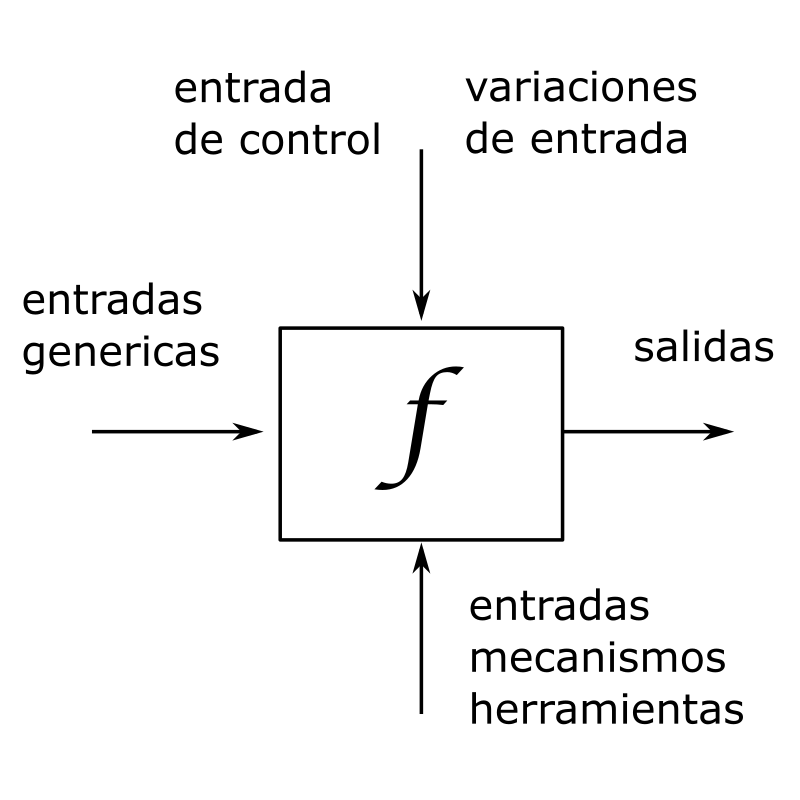
\includegraphics[scale=0.30]{Proyecto Integrador Figuras/15 IDEF0.png}
        \caption{IDEF-0}
 \end{figure}

\subsection{Modelo EFFBD}
Permite en la arquitectura funcional determinas el comportamiento que tiene un sistema a través del flujo de funciones. Este flujo está definido como el trayecto que siguen las entradas y salidas a lo largo de transformaciones.

\subsubsection{Generalidades}
Las funciones se representan con bloques, estos tienen un indicador (el mismo que se obtiene de la estructura funcional).

\begin{figure}[h!]
    \centering
        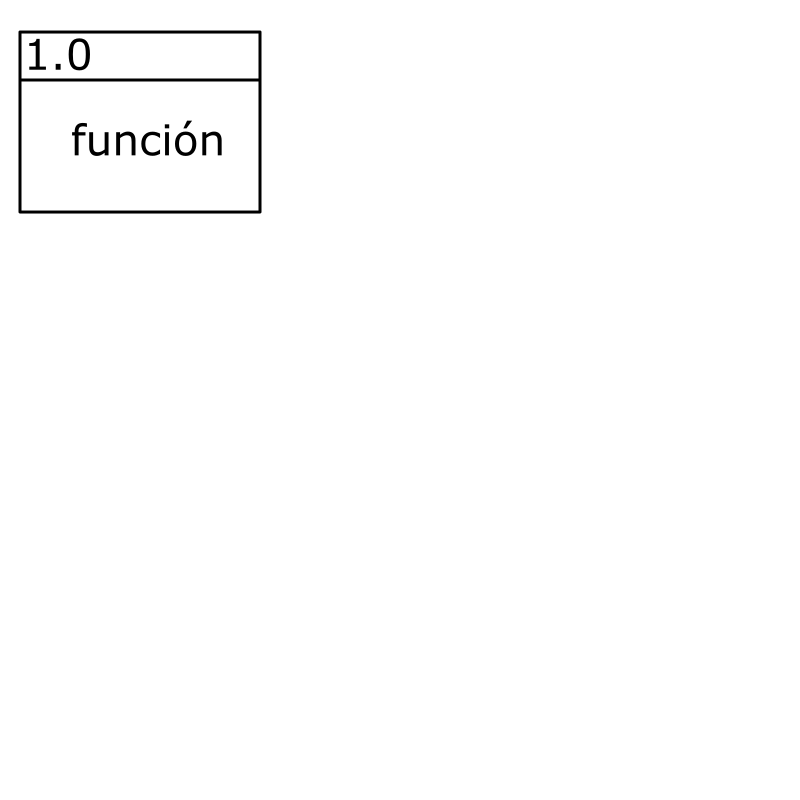
\includegraphics[scale=0.05]{Proyecto Integrador Figuras/16 Funcion.png}
        \caption{Función}
\end{figure}

Existen dos tipos de entradas y salidas, las entradas "pasivas" y las entradas "activas".

Las activas se refieren a que mantienen su flujo activo mientras se realiza la transformación. Las pasivas ya no transmiten flujo hasta que termine la transformación. 

\begin{figure}[h!]
    \centering
        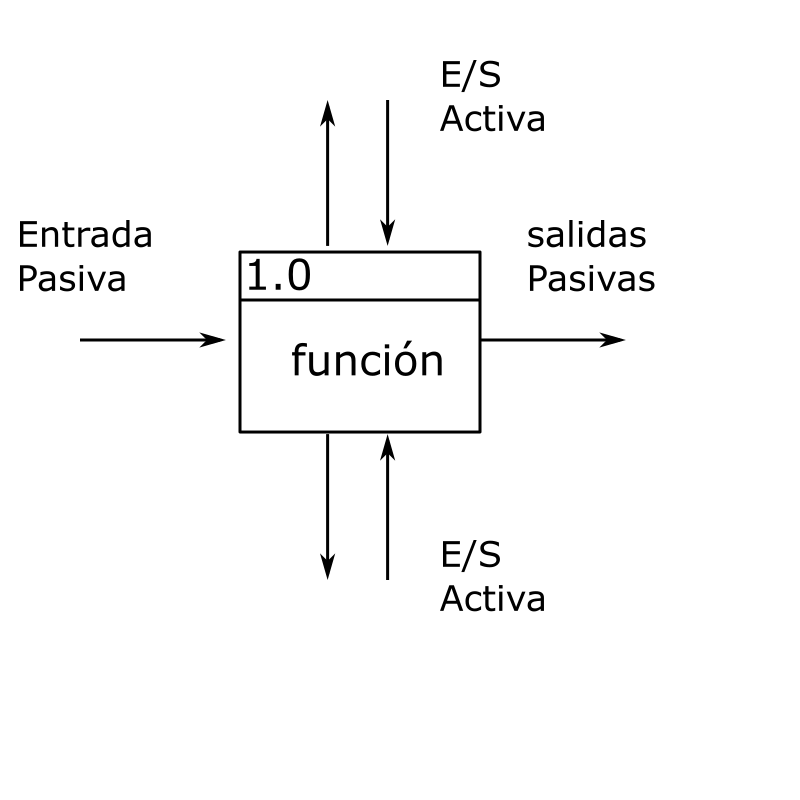
\includegraphics[scale=0.05]{Proyecto Integrador Figuras/17 Activas_Pasivas.png}
        \caption{Activas y pasivas}
\end{figure}

Para describir el comportamiento se tiene cuatro tipos de operadores lógicos.

\begin{enumerate}
    \item AND
    \item OR (paralelo), XOR (no se puede en paralelo)
    \item LOOP
    \item ITERACION
\end{enumerate}

\begin{figure}[h!]
    \centering
        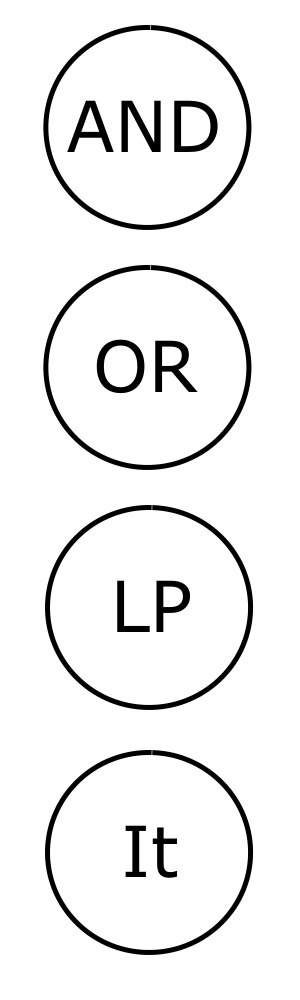
\includegraphics[scale=0.20]{Proyecto Integrador Figuras/18 Operadores.png}
        \caption{Operadores}
\end{figure}

Estos operadores se representan con un círculo y su símbolo se emplean deben aparecer al inicio y al fin de su uso. En el caso de los operadores "it" y "LP", se deben incluir la condición a la que están sujetas. 

Al inicio y al término del modelo se deben incluir funciones o acciones de referencias: se expresan como:

\begin{figure}[h!]
    \centering
        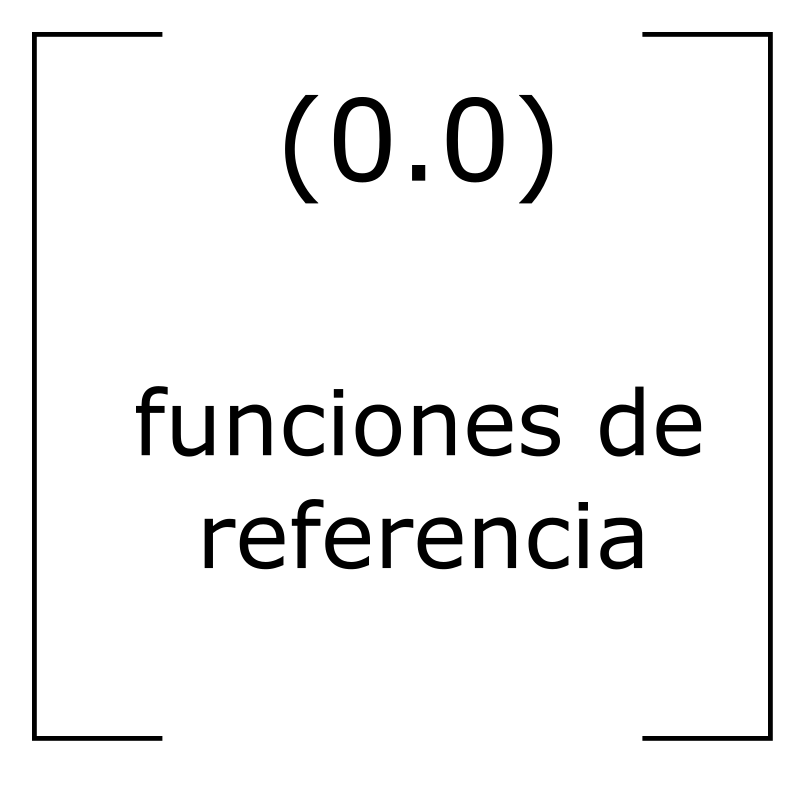
\includegraphics[scale=0.20]{Proyecto Integrador Figuras/19 Funciones de Referencia.png}
        \caption{Funciones de referencia}
\end{figure}

Existen otro tipo de funciones que son tentativas, es decir, no siempre existen. Estas se representan con bloques punteados. 

\begin{figure}[h!]
    \centering
        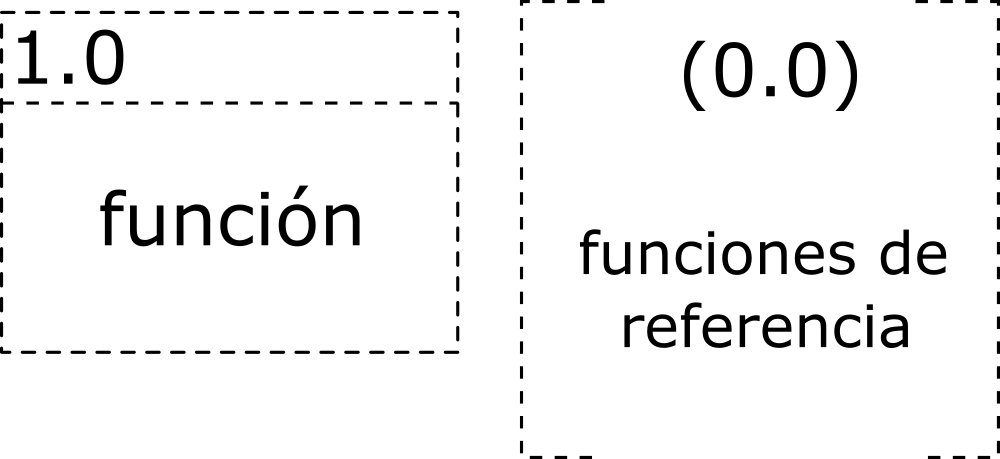
\includegraphics[scale=0.20]{Proyecto Integrador Figuras/20 Funciones Tentativas.png}
        \caption{Funciones tentativas}
\end{figure}

Si existieran elementos actuadores del comportamiento, estos se modelan con rectángulos con aristas redondeadas.

\begin{figure}[h!]
    \centering
        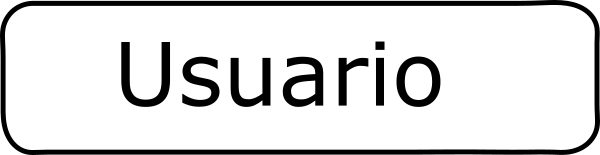
\includegraphics[scale=0.20]{Proyecto Integrador Figuras/21 Elementos Actuadores.png}
        \caption{Elementos actuadores}
\end{figure}

Para evaluación del diseño se emplea el coeficiente de diseño mecatrónico (MQD). Con los siguientes atributos.
\begin{enumerate}
    \item Inteligencia
    \item Robusto
    \item Flexible
    \item Adaptable
    \item Eficiencia del ensamble
\end{enumerate}